\documentclass[a4paper,ngerman,12pt]{zirkelblatt1415}

\usepackage[a4paper, left=3cm, right=3cm, top=3cm, bottom=3cm]{geometry}

\usepackage[utf8]{inputenc}

\usepackage[ngerman]{babel}

\usepackage{amsmath,amsthm,amssymb,stmaryrd,color,graphicx}
\usepackage{setspace}
\usepackage{bussproofs}
\usepackage{array}
\usepackage{comment,float,wrapfig}

\usepackage[protrusion=true,expansion=true]{microtype}

\usepackage{lmodern}

\usepackage{hyperref}

\setlength\parskip{\medskipamount}
\setlength\parindent{0pt}

\theoremstyle{definition}
\newtheorem{defn}{Definition}[section]
\newtheorem{axiom}[defn]{Axiom}
\newtheorem{bsp}[defn]{Beispiel}

\theoremstyle{plain}
\newtheorem{prop}[defn]{Proposition}
\newtheorem{motto}[defn]{Motto}
\newtheorem{wunder}[defn]{Wunder}
\newtheorem{ueberlegung}[defn]{??berlegung}
\newtheorem{lemma}[defn]{Lemma}
\newtheorem{kor}[defn]{Korollar}
\newtheorem{hilfsaussage}[defn]{Hilfsaussage}
\newtheorem{satz}[defn]{Satz}

\theoremstyle{remark}
\newtheorem{bem}[defn]{Bemerkung}
\newtheorem{aufg}[defn]{Aufgabe}

\newcommand{\RR}{\mathbb{R}}
\newcommand{\CC}{\mathbb{C}}
\newcommand{\ZZ}{\mathbb{Z}}
\renewcommand{\NN}{\mathbb{N}}
\newcommand{\QQ}{\mathbb{Q}}
%\newcommand{\K}{\mathbb{K}}
\newcommand{\PP}{\mathbb{P}}
%\newcommand{\CP}{\mathbb{CP}}
%\newcommand{\RP}{\mathbb{RP}}
\newcommand {\kk} {\Bbbk}
\newcommand{\VV}{\mathbb V}
\newcommand{\HH}{\mathbb{H}}
\newcommand{\ii}{\mathrm{i}}
\newcommand{\AM}{\operatorname{AM}}
\newcommand{\GM}{\operatorname{GM}}
\newcommand{\HM}{\operatorname{HM}}
\newcommand{\QM}{\operatorname{QM}}

\renewcommand{\Re}{\operatorname{Re}}
\renewcommand{\Im}{\operatorname{Im}}

\newcommand{\lra}{\longrightarrow}
\newcommand{\ol}[1]{\overline{#1}}

\setlength\unitlength{1cm}

% \RequirePackage{geometry}
% \geometry{textwidth=16.0cm,textheight=24.5cm,footskip=1.5cm}

%\usepackage{tikz,braids}
%\usetkzobj{all}
%\usetikzlibrary{calc,shapes,arrows,positioning}

\begin{document}

%\maketitle{Zwergenr??tsel}{}

\begin{center}
  \textbf{\Large Zwergenr??tsel}
\end{center}



\begin{enumerate}
  \item Gregor strandet auf einer von zwei benachbarten Inseln. Die Zwerge der einen Insel l??gen stets, die der anderen sagen immer die Wahrheit. Gregor m??chte mit nur einer Ja/Nein-Frage herausfinden, ob er sich auf der Wahrheits- oder der L??geninsel befindet. Da sich die Zwerge gegenseitig besuchen, wei?? Gregor noch nicht einmal, von welcher Insel der Zwerg, den er anspricht, eigentlich stammt. Was kann Gregor fragen?

\begin{figure}[H]
  \centering
  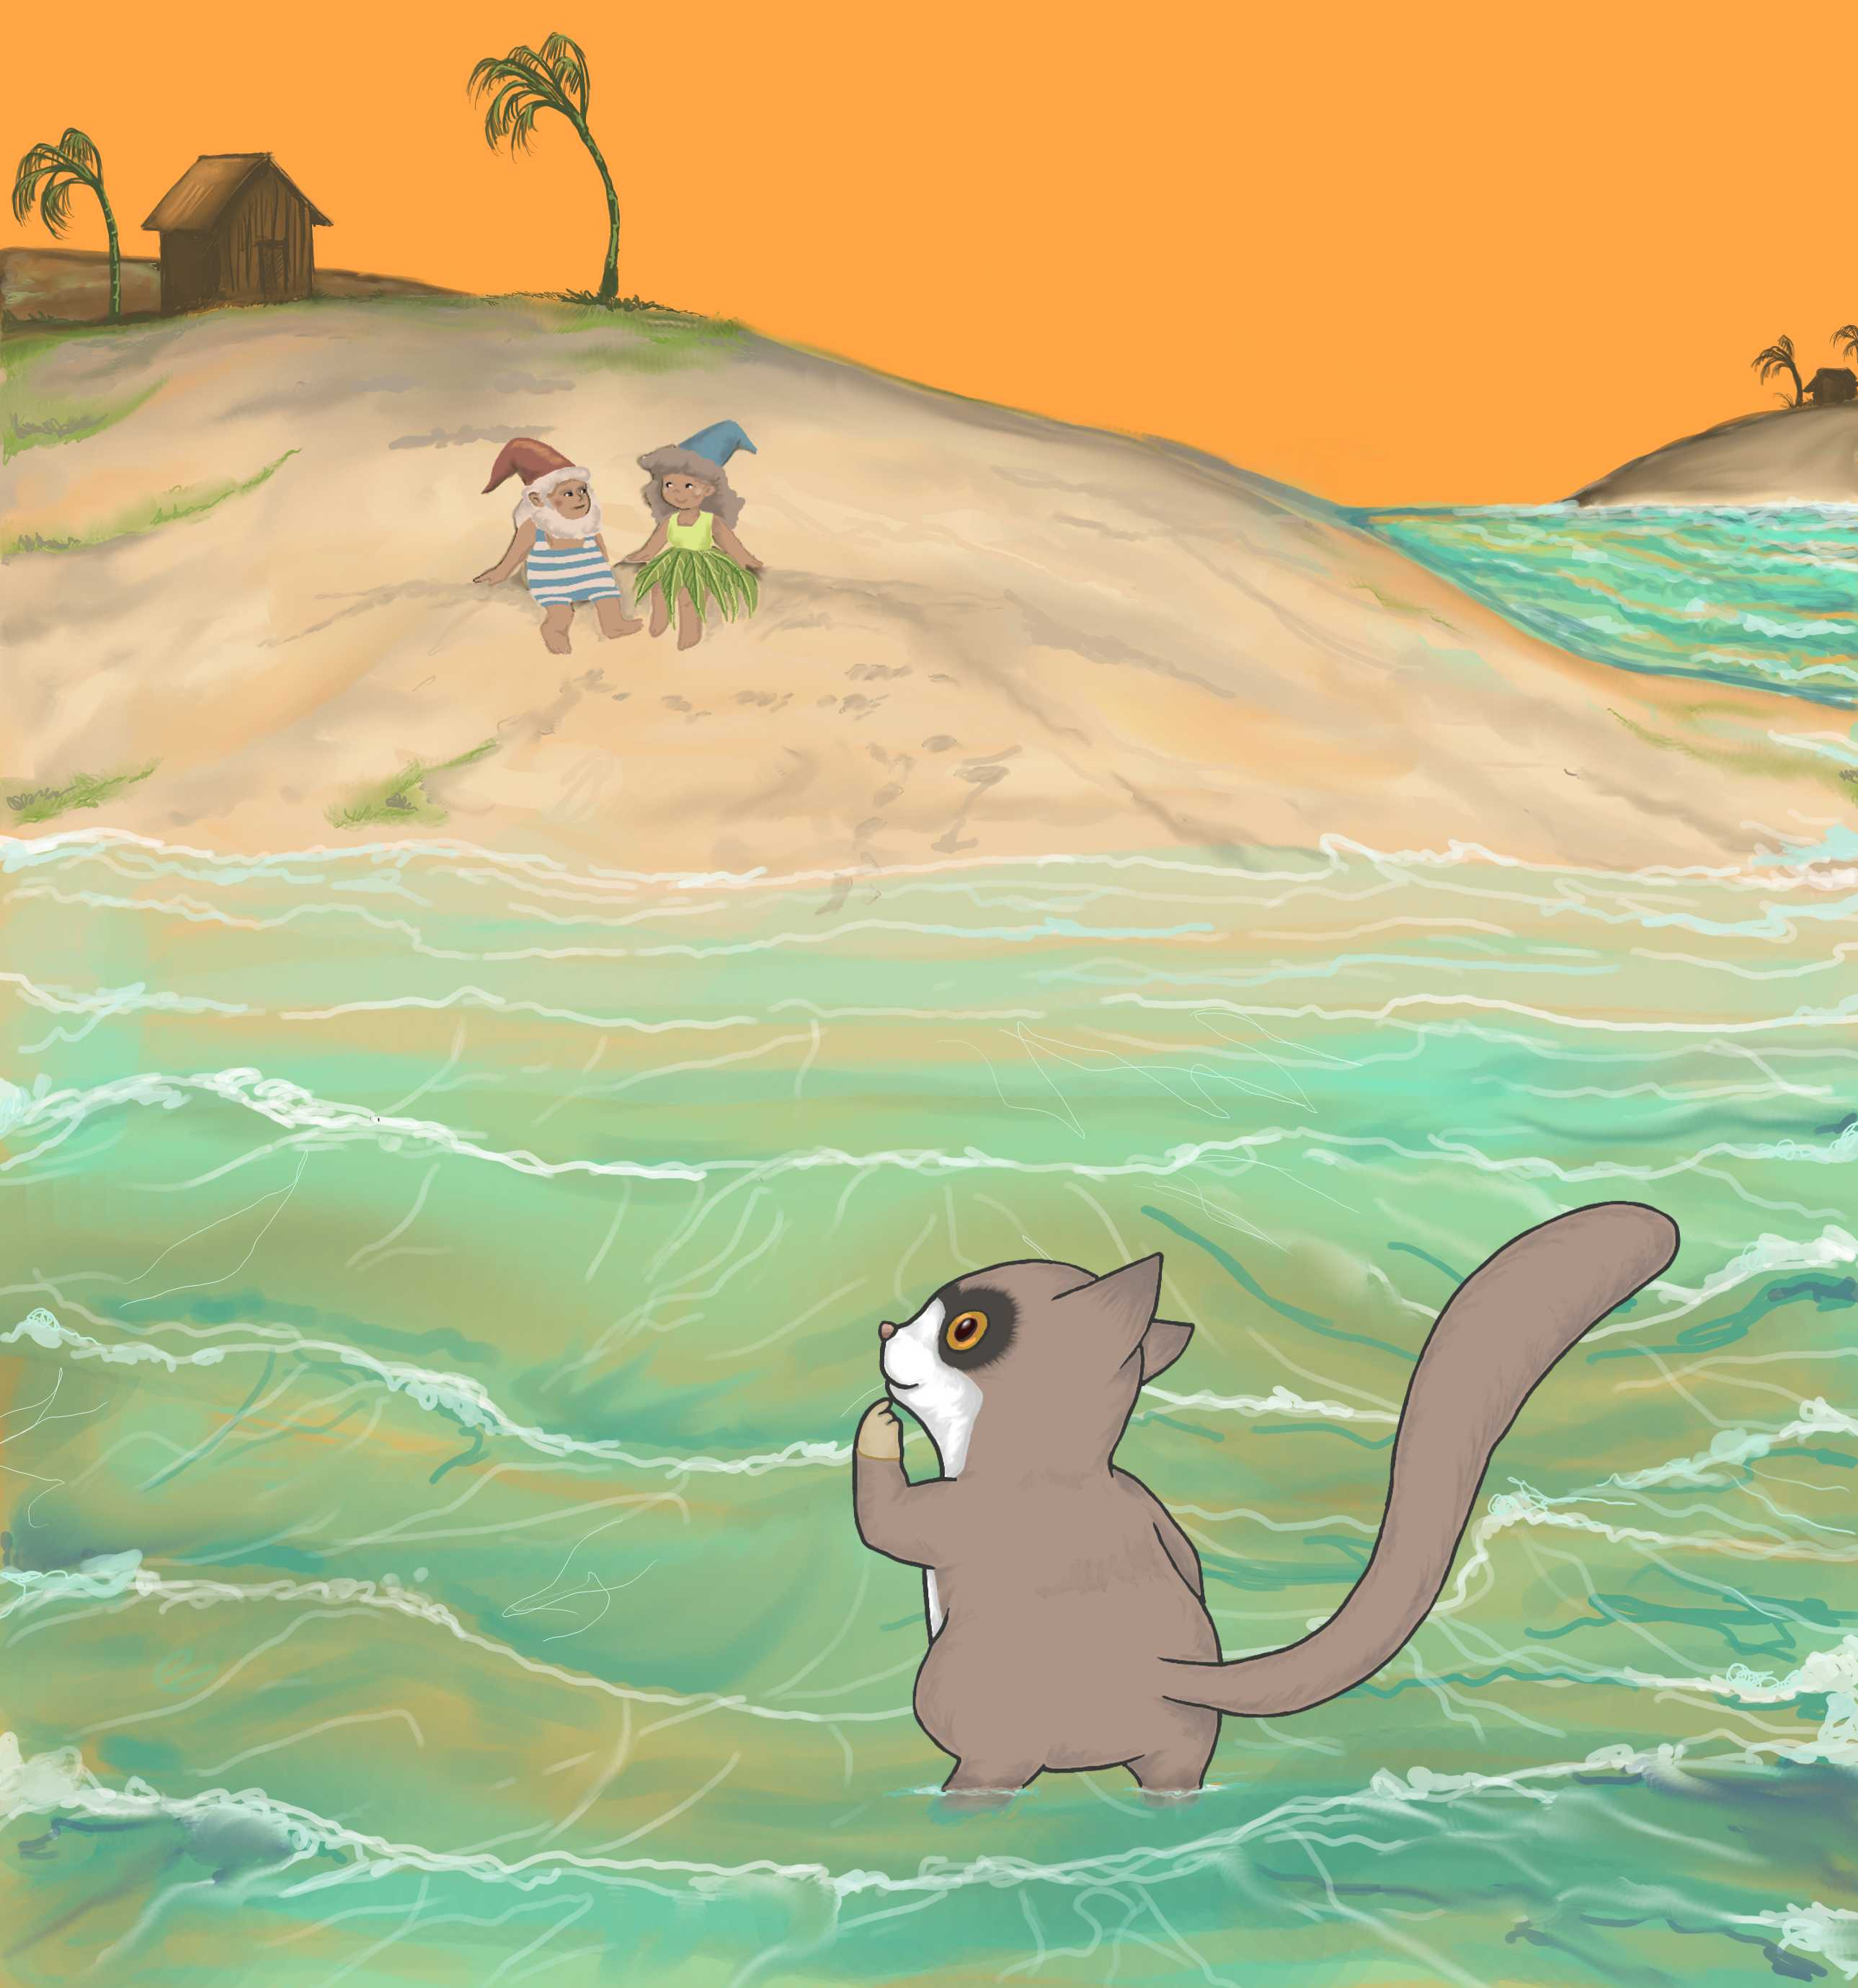
\includegraphics[width=0.3\textwidth]{bilder/gregor-strand.jpg}
\end{figure} 

  \item Auf einem ein Meter langen Stab stehen einhundert Zwerge. Jeder bewegt sich mit genau einem Zentimeter pro Sekunde. Anfangs schaut jeder Zwerg in eine bestimmte Richtung. Sobald zwei Zwergen aufeinander sto??en, kehren sie um und laufen in die jeweils andere Richtung weiter. Wie lange dauert es h??chstens, bis alle Zwerge das Ende des Stabs erreicht haben? (Dort fallen sie dann herunter und geh??ren nicht mehr zum Spiel.)
  \item In einem einsamen Bergdorf gibt es 20 Zwerge. Eines Tages kommt der b??se Riese vorbei und l??sst die Zwerge in einer Reihe aufstellen, sodass jeder nur noch die Zwerge vor ihm sieht. Danach setzt der Riese jedem Zwerg entweder eine rote oder eine blaue Zipfelm??tze auf den Kopf. Jeder Zwerg darf jetzt nacheinander eine Farbe sagen, wobei der Zwerg, der alle anderen 19 Zwerge vor ihm sieht, beginnen muss. Wenn ein Zwerg die Farbe seiner Zipfelm??tze err??t, kommt er frei, sagt er jedoch die falsche Farbe, muss er zwei Wochen f??r den Riesen auf dem Feld arbeiten. Mit welcher Strategie k??nnen die Zwerge m??glichst viele (wieviele?) vor der Zwangsarbeit bewahren?
  \item (*) 100 Zwerge haben H??te aufgesetzt bekommen, die zwar alle die gleiche Farbe haben, aber mit einer nat??rlichen Zahl zwischen einschlie??lich $0$ und $99$ beschriftet sind. Die Zahlen k??nnen nach irgendeinem System geordnet sein oder auch v??llig zuf??llig verteilt sein. Es kann auch sein, dass manche Zahlen mehrmals und andere gar nicht vorkommen. Jeder Zwerg sieht die Zahlen der anderen Zwerge, aber nicht seine eigene. Auf Zuruf m??ssen dann alle Zwerge gleichzeitig eine Zahl zwischen $0$ und $99$ nennen. Stimmt sie mit der eigenen Hutzahl ??berein, erh??lt der betreffende Zwerg ein Bonbon und sonst nicht. Mit welcher Strategie k??nnen die Zwerge erreichen, dass mindestens ein Zwerg sicher ein Bonbon erh??lt?

% \begin{figure}[H]
%   \centering
%   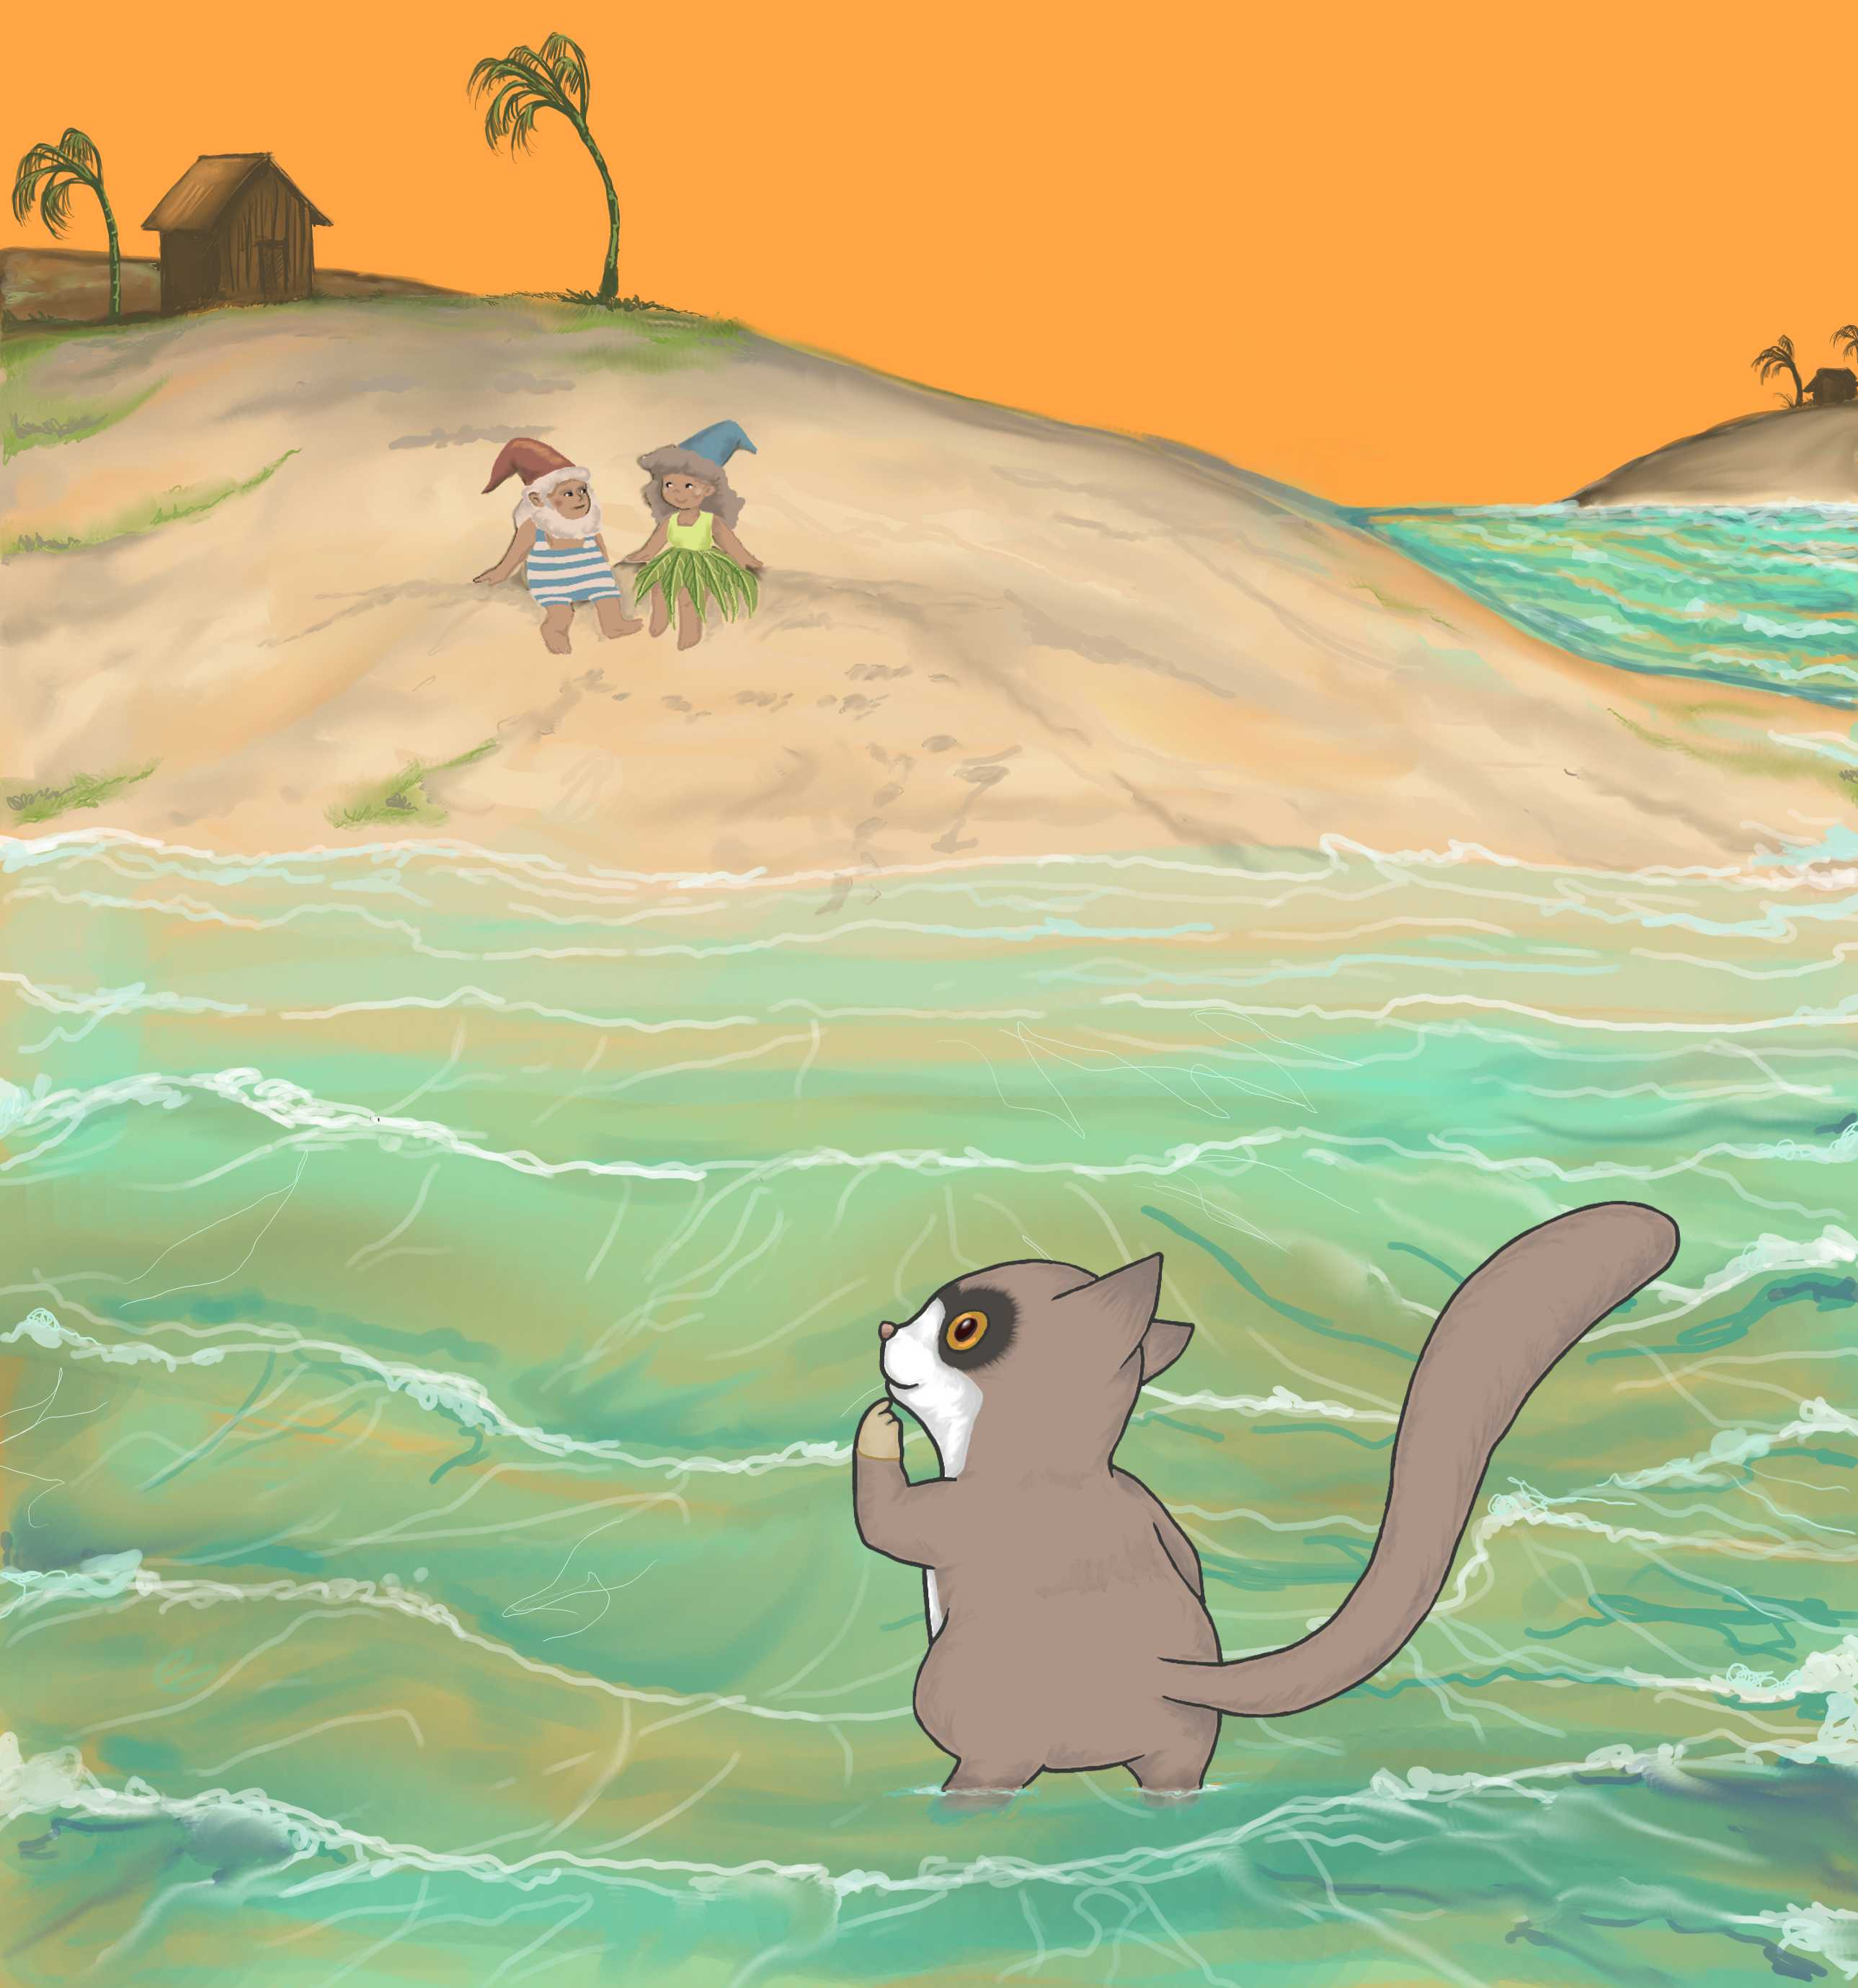
\includegraphics[width=0.3\textwidth]{bilder/gregor-strand.jpg}
% \end{figure}

  \item Drei Zwerge stehen mit je einem gelben oder roten Hut auf dem Kopf im Kreis. Sie k??nnen also die Hutfarben der anderen, nicht aber ihre eigene sehen. Man teilt ihnen mit, dass mindestens ein Hut rot ist. Der erste wird gefragt, ob er die Farbe seines Huts wei??; er verneint. Der zweite wird gefragt, ob er die Farbe seines Huts wei??; auch er verneint. Was ist die Farbe des Hutes des dritten Zwerges?
  \item $100$ Zwerge haben zwei verschiedene Farben von M??tzen auf. Sie werden einzeln in einen Raum gef??hrt, in dem sie sich in einer Reihe nach Farben sortiert aufstellen sollen. Wie machen sie das, wenn sie vorher eine Strategie ausmachen d??rfen, w??hrenddessen aber nicht reden d??rfen und nur die M??tzenfarben der anderen, aber nicht ihre eigenen, sehen?
  \item $32$ Zwerge sitzen in einem Kreis und haben rote und wei??e M??tzen auf. Dabei ist bekannt, dass nicht alle M??tzen wei?? sind. Jetzt sollen alle Zwerge gleichzeitig sagen, welche Farbe ihre M??tze hat. K??nnen sie erreichen, dass mindestens einer der Zwerge die richtige Anzahl sagt? K??nnen sie auch erreichen, dass mehr Zwerge die richtige Anzahl sagen?
  \item (*) Die b??sen Trolle haben unendlich viele Zwerge versammelt und wieder H??te der Farben Schwarz und Wei?? aufgesetzt. Alle Zwerge k??nnen sich gegenseitig sehen, nur ihre eigene Hutfarbe bleibt ihnen verborgen. Auf Kommando m??ssen dann alle Zwerge jeweils "`schwarz"' oder "`wei??"' rufen. Wer damit seine eigene Hutfarbe err??t, bleibt am Leben; andernfalls wird er umgebracht. Vorab d??rfen die Zwerge eine Strategie ausmachen, danach aber ist jede Kommunikation verboten. Finde eine Strategie, mit der auf jeden Fall \emph{alle bis auf endlich viele} Zwerge ??berleben!\footnote{Achtung: Das ist eine st??rkere Anforderung als nur zu verlangen, dass \emph{unendlich viele} Zwerge ??berleben. Wenn zum Beispiel jeder zweite Zwerg ??berlebt, dann ??berleben zwar unendlich viele Zwerge, aber es sterben auch unendlich viele.}
  \item (*) Wie ??blich wurden 100 Zwerge (mit den Nummern $1, 2, \ldots, 100$) gefangen genommen. Der Gef??ngnischef erkl??rt die Regeln:

Die Zwerge werden, jeder f??r sich, in einen Raum gef??hrt. In diesem Raum befinden sich 100 Schubladen (durchnummeriert von $1$ bis $100$). In jeder der Schubladen befindet sich ein Zettel. Auf den Zetteln steht jeweils eine Nummer von $1$ bis $100$. Jede Nummer steht auf genau einem Zettel, es kommt also nicht zu Wiederholungen.

Jeder Zwerg darf nun f??nfzig Schubladen seiner Wahl ??ffnen. Entdeckt er dabei den Zettel mit seiner eigenen Nummer, ist alles gut. Entdeckt er seinen eigene Nummer dagegen nicht, so sterben alle (!) Zwerge.

Schafft jeder Zwerg, seine Nummer zu finden, so kommen alle Zwerge frei. Die Zwerge k??nnen sich vorab auf eine Strategie einigen, ab Beginn des "`Spiels"' aber nicht mehr miteinander kommunizieren. Den Raum mit den Schubladen m??ssen sie genau so verlassen, wie sie ihn vorgefunden haben.

Die Frage lautet: Gibt es eine Strategie, sodass die Zwerge nicht nur mit verschwindend geringer Wahrscheinlichkeit ??berleben und freigelassen werden?

\begin{figure}[H]
  \centering
  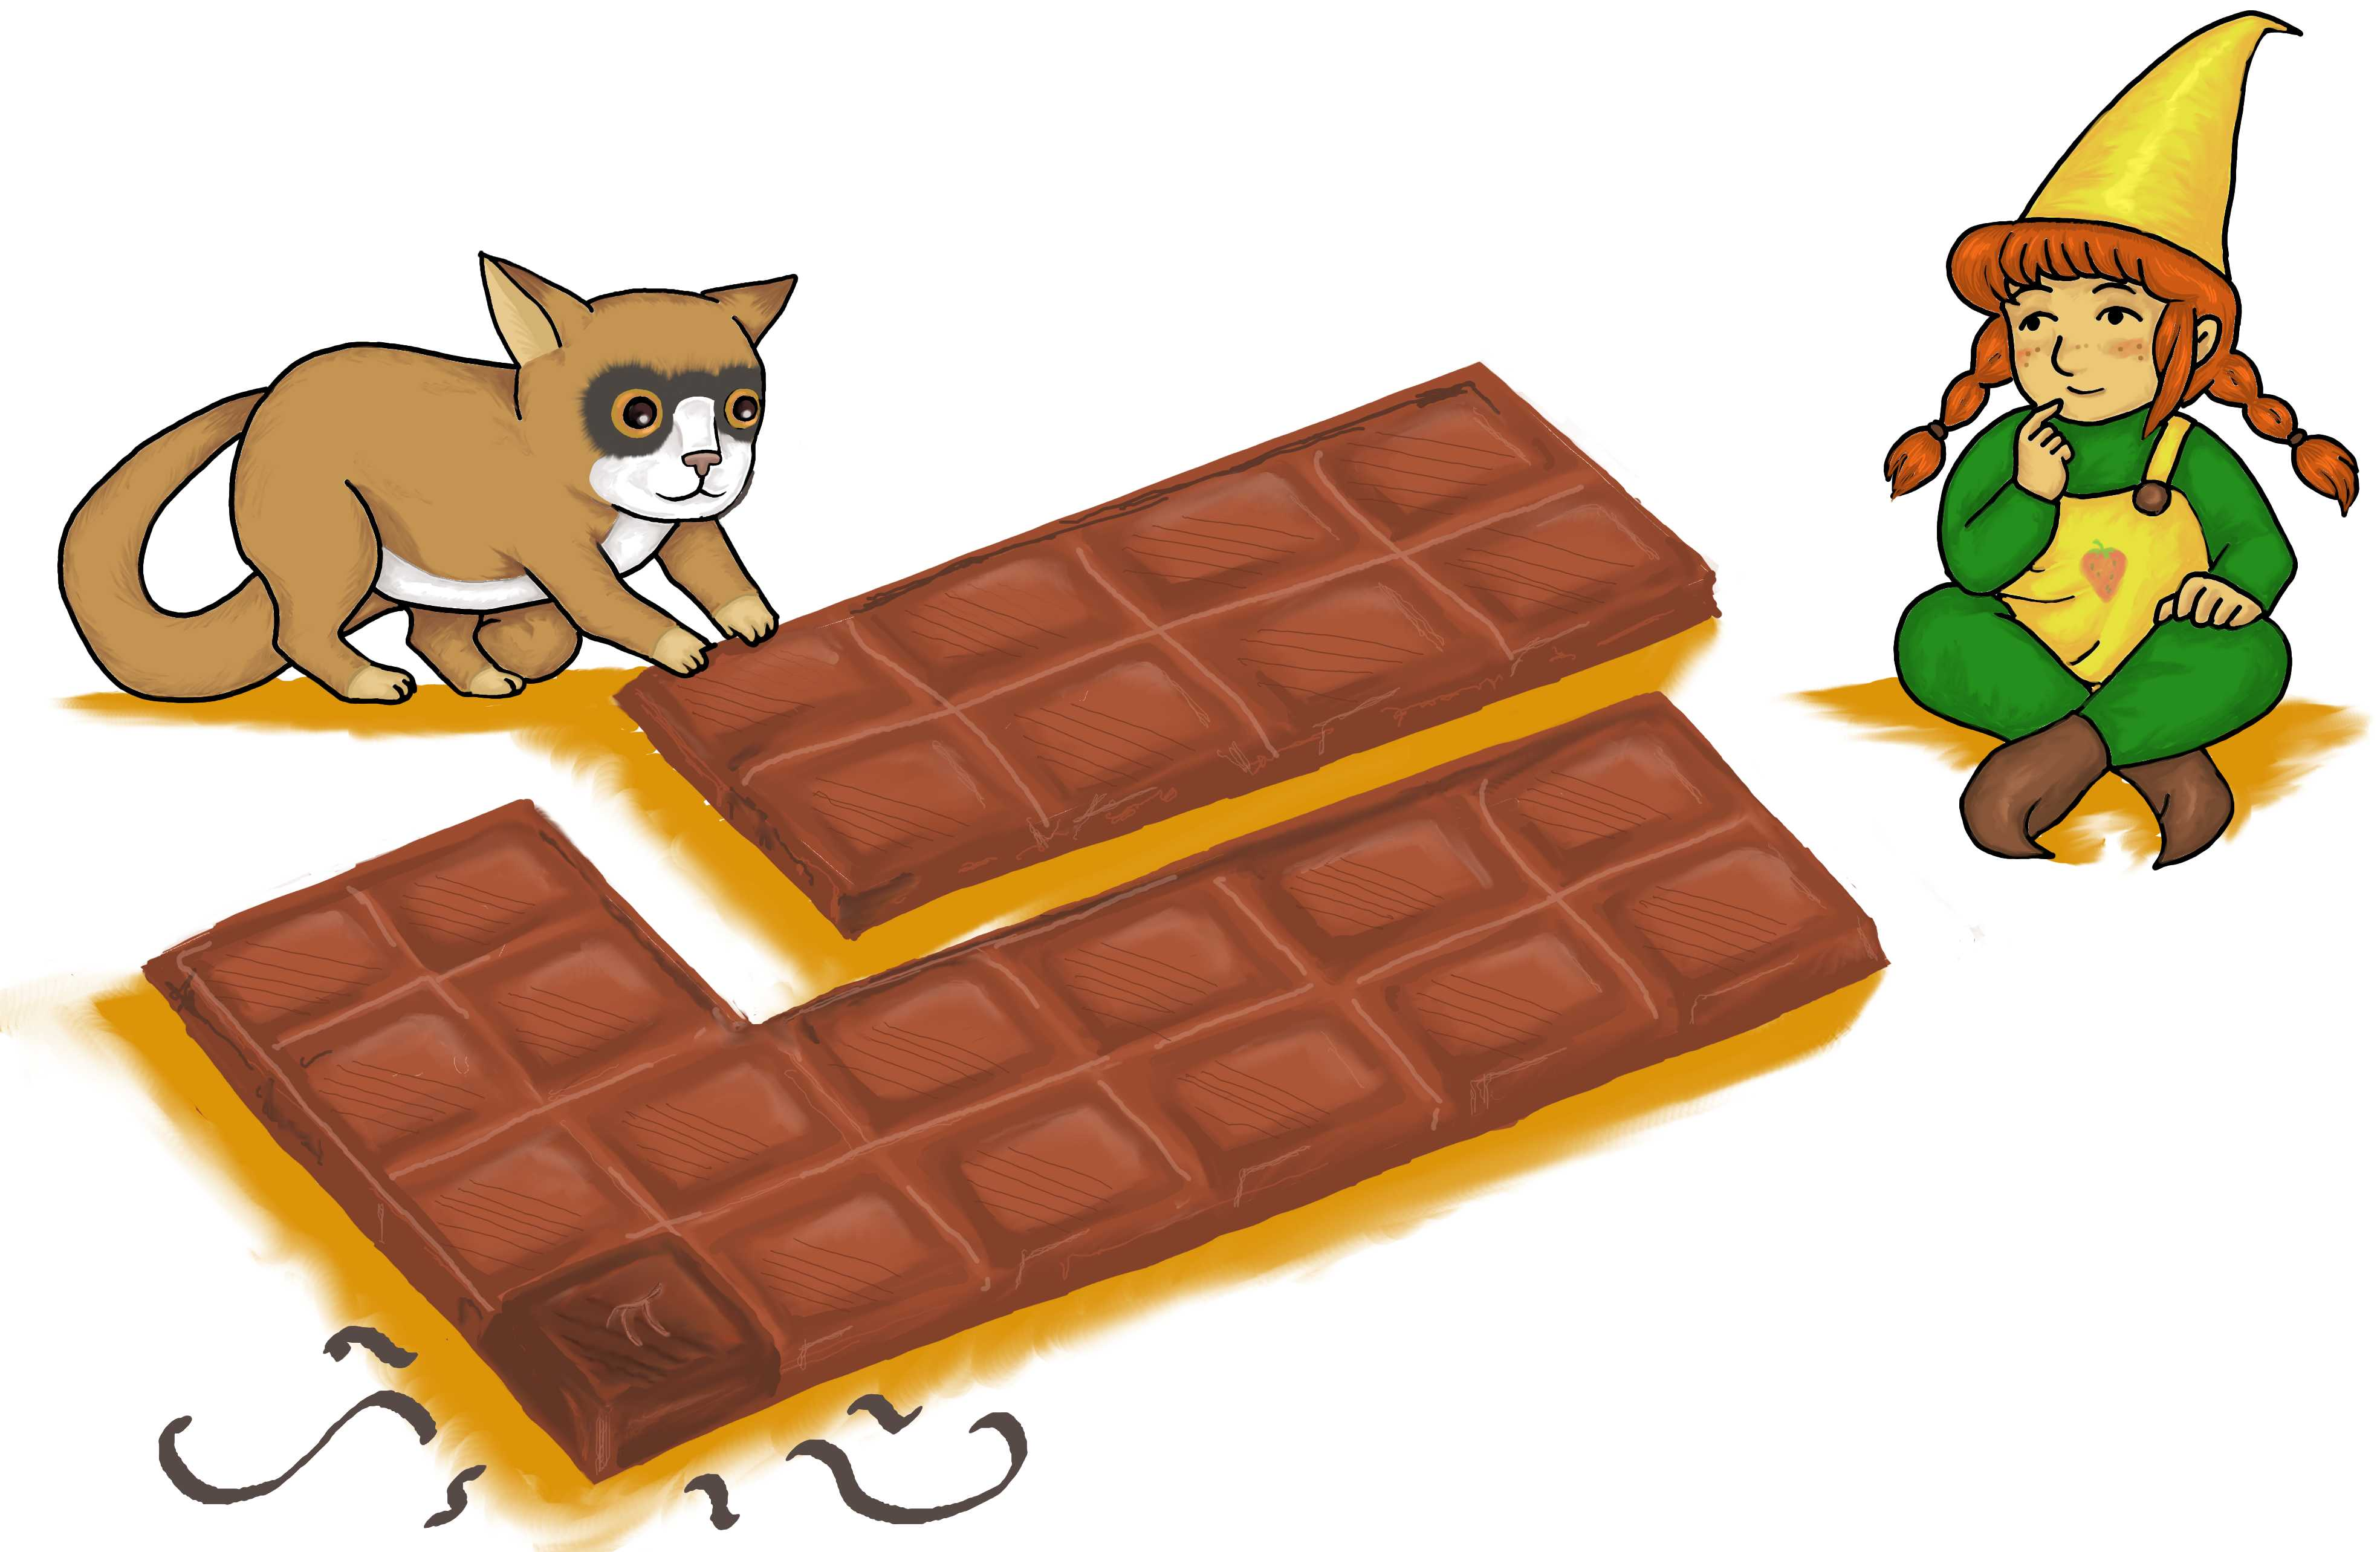
\includegraphics[width=0.5\textwidth]{bilder/schoko.jpg}
\end{figure} 

  \item (*) Eine Zwergenschule hat $100$ Sch??lerinnen und Sch??ler. Jeden Tag wird zuf??llig ein Zwerg zum Riesendirektor gerufen. Der Zwerg darf dann behaupten, dass zu diesem Zeitpunkt schon alle Zwerge mindestens einmal beim Riesen waren. Stimmt das, so d??rfen alle zum Mathecamp mitfahren. Stimmt das nicht, darf niemand jemals wieder mitkommen. Zur Kommunikation dient eine einzige Lampe im Riesenb??ro, die an oder aus sein kann. Die Zwerge d??rfen den Status dieser Lampe bei ihren Riesenbesuchen ??ndern (m??ssen aber nicht). Der Riese r??hrt die Lampe nicht an. Die Zwerge sehen nicht, welche anderen Zwerge bereits beim Riesen waren. Ein und derselbe Zwerg kann m??glicherweise mehrere Male zum Riesen gerufen werden. Finde eine Strategie, mit der die Zwerge schlussendlich wieder sicher zum Mathecamp d??rfen!\footnote{Kommunikation ist nat??rlich nur vorher erlaubt. Es geht nicht um Restw??rme der Lampe oder ??hnliches. Die zuf??llige Reihenfolge des Riesendirektors ist so, dass jede endliche Folge von Zwergen irgendwann einmal vorkommt.}
  \item Auf einer einsamen Insel leben $100$ Zwerge, von denen jeder genau eine von zwei Augenfarben hat -- entweder Gr??n oder Blau. Dies ist allen bekannt. Jedoch hat sich bei den Zwergen folgendes Ritual etabliert: Sobald ein Zwerg wei??, dass seine eigene Augenfarbe Blau ist, verl??sst er die Insel in der darauffolgenden Nacht. Einmal am Tag treffen sich die Zwerge, sodass jeder Zwerg die Augenfarben aller anderen Zwerge sieht.\footnote{Zwerge leben ??brigens f??r immer, werden niemals neu geboren, kommen auch niemals neu auf die Insel und sind sehr sehr schlau.} Da niemand die Insel verlassen will, schaut niemand in irgendwelche Spiegel oder ??hnliches und man redet nicht ??ber die Augenfarbe. Eines Tages kommt Gregor auf die Insel und erz??hlt den Zwergen, dass es einen Zwerg mit blauen Augen gibt. Nach wievielen Tagen sind alle Zwerge mit blauen Augen sp??testens weg und warum?
\end{enumerate}

\begin{figure}[H]
  \centering
  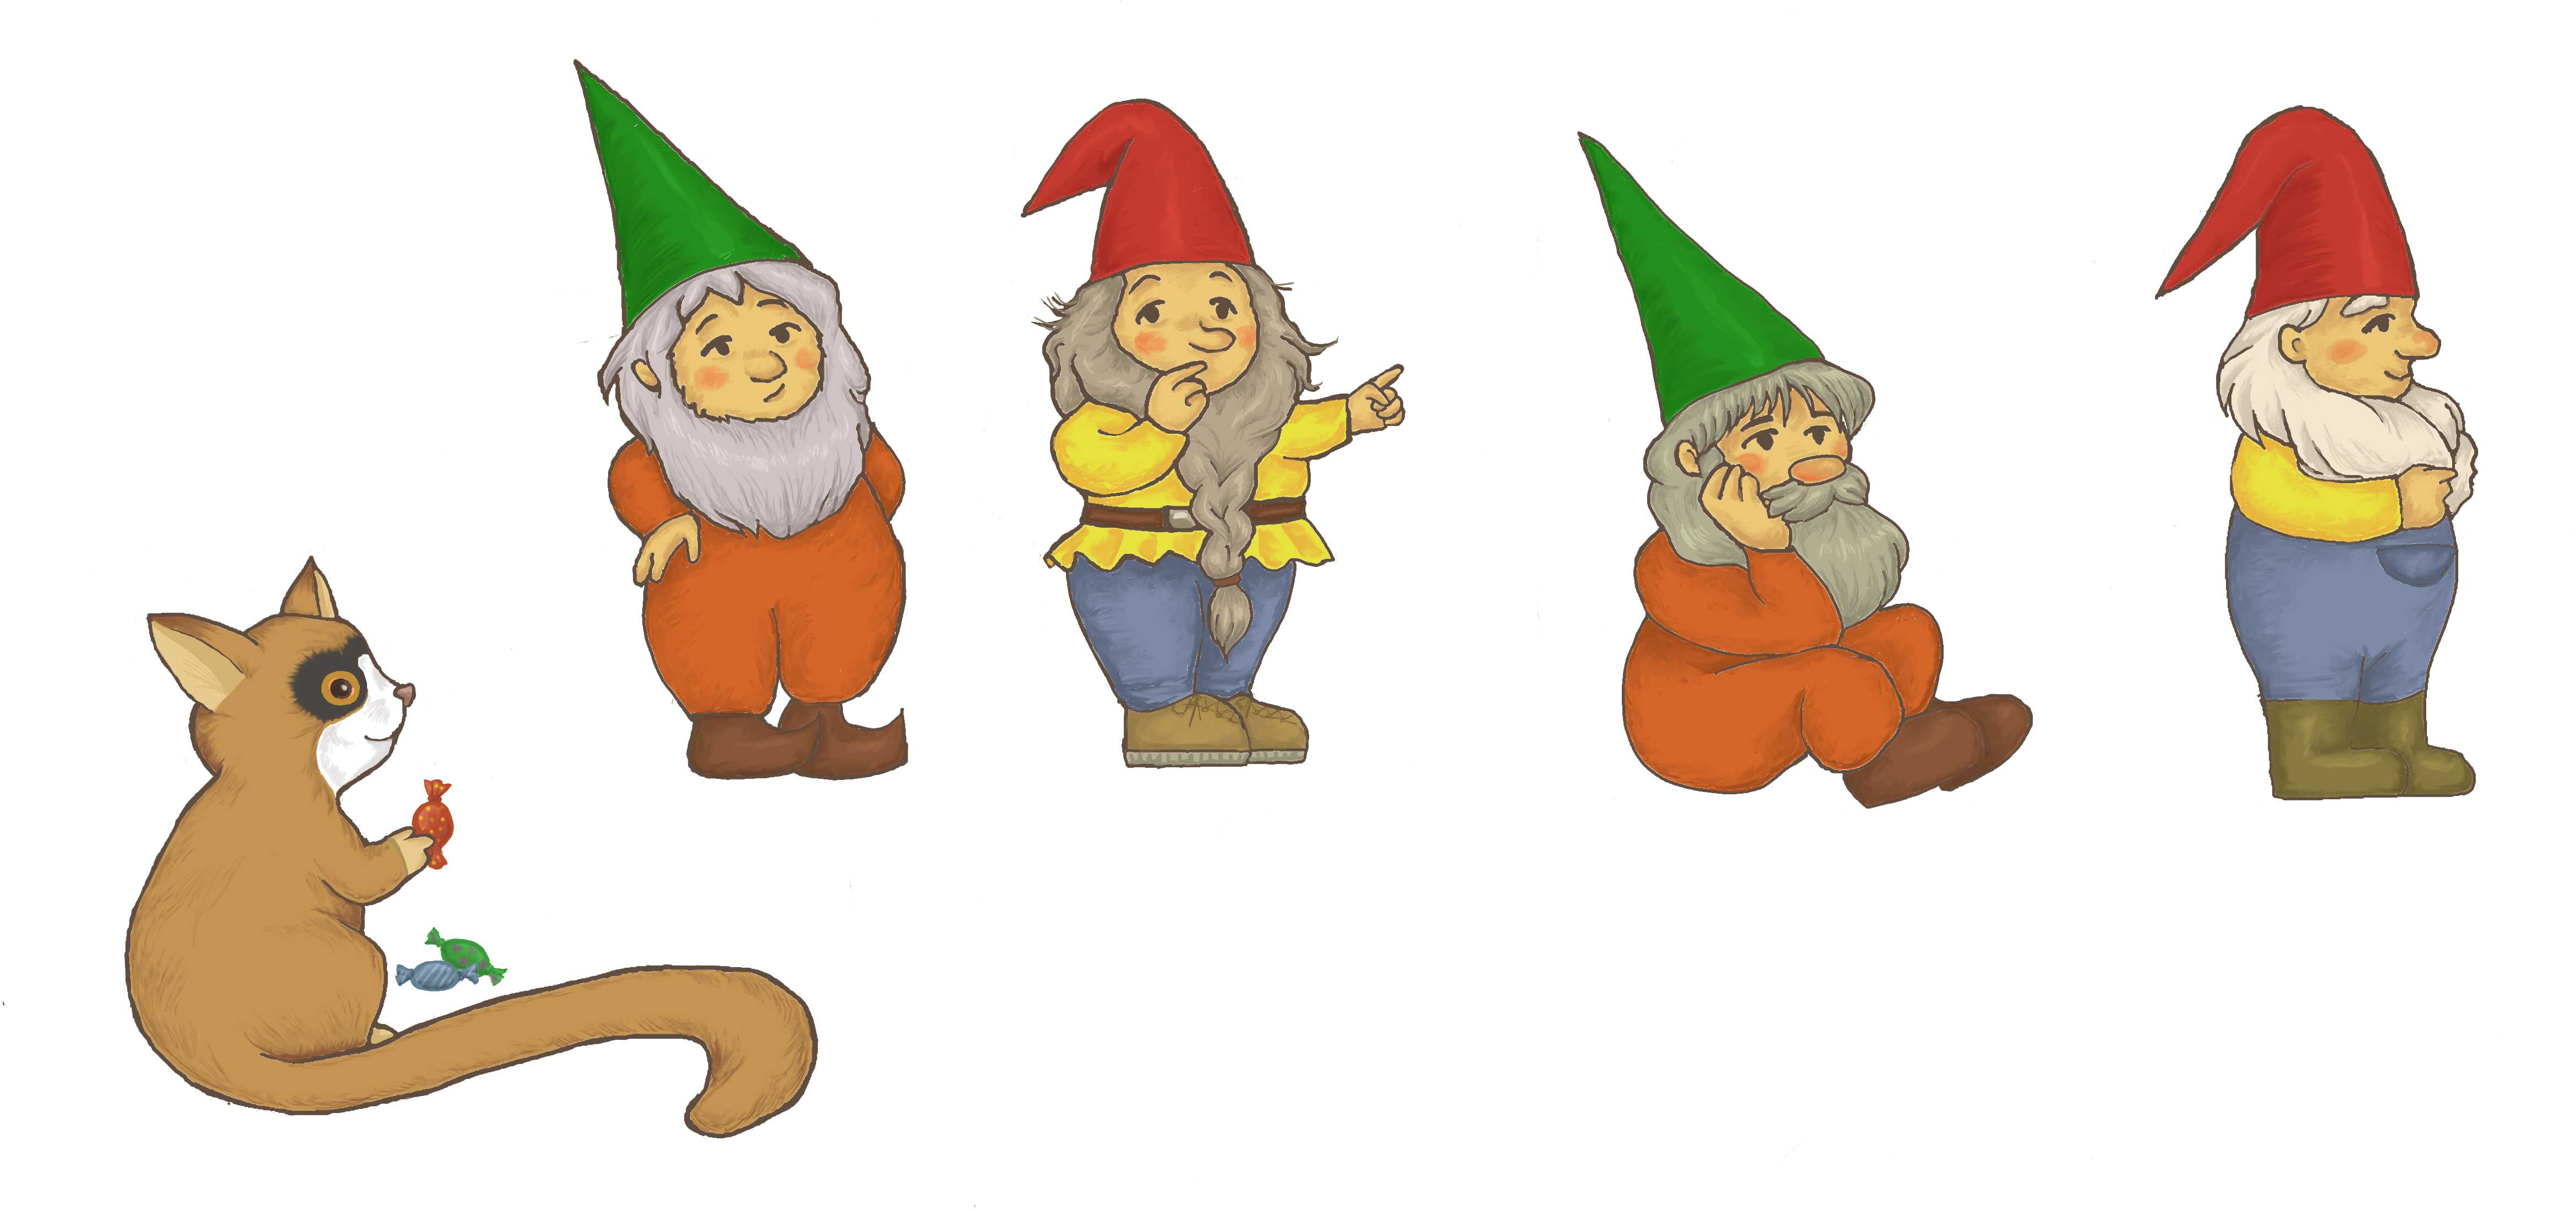
\includegraphics[width=0.8\textwidth]{bilder/aufgabe-zwerge.jpg}
\end{figure}

\begin{enumerate}
\setcounter{enumi}{11}
\item (*) Ein Riese schreibt zwei beliebige, verschiedene ganze Zahlen auf zwei Zettel und legt sie nebeneinander verdeckt auf den Tisch. Ein Zwerg darf nun einen der beiden Zettel aufdecken und sich die Zahl anschauen. Er kann dann entweder bei seiner Wahl bleiben oder den anderen Zettel ausw??hlen. Er gewinnt, wenn er den Zettel mit der gr????eren der beiden Zahlen ausgew??hlt hat. Gibt es eine Strategie, die dem Kandidat erlaubt, mit Wahrscheinlichkeit gr????er als 50\% zu gewinnen?
\end{enumerate}

\end{document}